% Replaces \section{Method} in sec/2_formatting.tex.
% The figure environment from the current draft is retained; panel (a) gains a
% fourth policy row (see PLAN.md §5) and the caption below is rewritten for it.

\section{Method}
\label{sec:method}

\begin{figure}[t]
\centering
\resizebox{\columnwidth}{!}{%
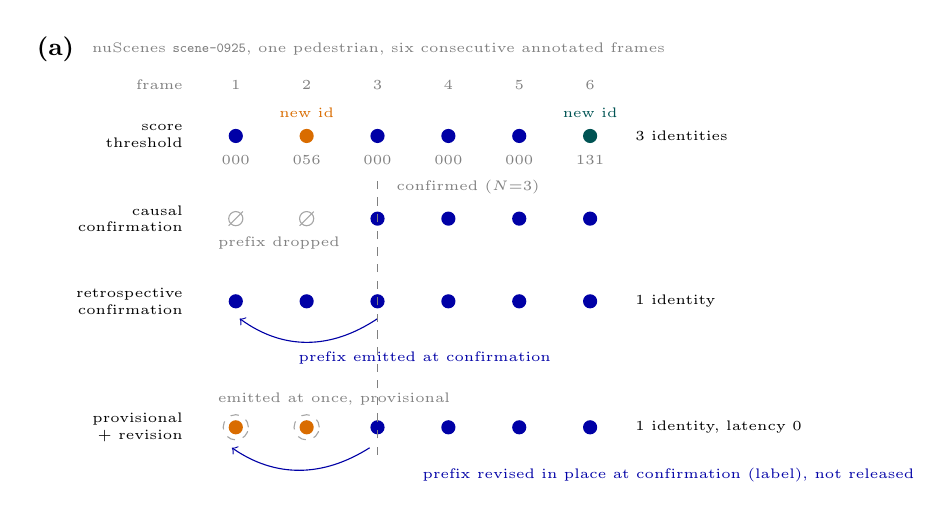
\begin{tikzpicture}
  \node[font=\small\bfseries, anchor=west] at (-1.75, 3.2) {(a)};
  \node[font=\tiny, gray, anchor=west] at (-1.05, 3.2) {nuScenes \texttt{scene-0925}, one pedestrian, six consecutive annotated frames};
  \foreach \x in {1,...,6} {\node[font=\tiny, gray] at (\x*0.9, 2.75) {\x};}
  \node[font=\tiny, gray, anchor=east] at (0.35, 2.75) {frame};
  % row 1: score threshold -- measured identities
  \node[anchor=east, align=right, font=\tiny] at (0.35, 2.1) {score\\threshold};
  \foreach \x in {1,3,4,5} {\fill[blue!65!black] (\x*0.9, 2.1) circle (0.09);}
  \fill[orange!85!black] (1.8, 2.1) circle (0.09);
  \fill[teal!65!black] (5.4, 2.1) circle (0.09);
  \foreach \x/\lab in {1/000, 2/056, 3/000, 4/000, 5/000, 6/131} {
    \node[font=\tiny, gray] at (\x*0.9, 1.79) {\lab};}
  \node[font=\tiny, orange!85!black] at (1.8, 2.40) {new id};
  \node[font=\tiny, teal!65!black] at (5.4, 2.40) {new id};
  \node[font=\tiny, anchor=west] at (5.85, 2.1) {3 identities};
  % row 2: causal confirmation
  \node[anchor=east, align=right, font=\tiny] at (0.35, 1.05) {causal\\confirmation};
  \foreach \x in {1,2} {
    \draw[gray!70] (\x*0.9, 1.05) circle (0.09);
    \draw[gray!70] (\x*0.9-0.09, 1.05-0.09) -- (\x*0.9+0.09, 1.05+0.09);}
  \foreach \x in {3,...,6} {\fill[blue!65!black] (\x*0.9, 1.05) circle (0.09);}
  \node[font=\tiny, gray, anchor=west] at (0.55, 0.74) {prefix dropped};
  % row 3: retrospective confirmation
  \node[anchor=east, align=right, font=\tiny] at (0.35, 0.0) {retrospective\\confirmation};
  \foreach \x in {1,...,6} {\fill[blue!65!black] (\x*0.9, 0.0) circle (0.09);}
  \node[font=\tiny, anchor=west] at (5.85, 0.0) {1 identity};
  \draw[->, blue!65!black] (2.7, -0.22) .. controls (2.1, -0.62) and (1.5, -0.62) .. (0.95, -0.22);
  \node[font=\tiny, blue!65!black] at (3.3, -0.72) {prefix emitted at confirmation};

  % row 4: provisional emission + revision (ours)
  \node[anchor=east, align=right, font=\tiny] at (0.35, -1.6) {provisional\\${+}$ revision};
  \foreach \x in {1,2} {\fill[orange!85!black] (\x*0.9, -1.6) circle (0.09);
                        \draw[dashed, gray!70] (\x*0.9, -1.6) circle (0.16);}
  \foreach \x in {3,...,6} {\fill[blue!65!black] (\x*0.9, -1.6) circle (0.09);}
  \node[font=\tiny, anchor=west] at (5.85, -1.6) {1 identity, latency 0};
  \draw[->, blue!65!black] (2.6, -1.86) .. controls (2.0, -2.24) and (1.4, -2.24) .. (0.85, -1.86);
  \node[font=\tiny, blue!65!black, anchor=west] at (3.15, -2.20)
       {prefix revised in place at confirmation (label), not released};
  \node[font=\tiny, gray, anchor=west] at (0.55, -1.24) {emitted at once, provisional};
  % confirmation marker
  \draw[dashed, gray] (2.7, -1.95) -- (2.7, 1.55);
  \node[font=\tiny, gray, anchor=west] at (2.82, 1.45) {confirmed ($N{=}3$)};
\end{tikzpicture}}
\\[4pt]
\resizebox{0.92\columnwidth}{!}{%
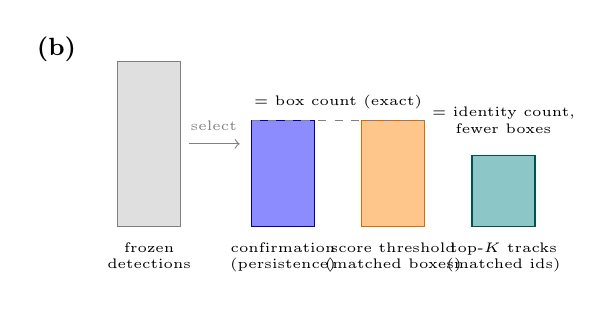
\begin{tikzpicture}
  \node[font=\small\bfseries, anchor=west] at (-1.15, 2.25) {(b)};
  \draw[fill=gray!25, draw=gray] (0, 0) rectangle (0.8, 2.1);
  \node[align=center, font=\tiny, anchor=north] at (0.4, -0.08) {frozen\\detections};
  \draw[->, gray] (0.9, 1.05) -- (1.55, 1.05);
  \node[font=\tiny, gray] at (1.22, 1.28) {select};
  \draw[fill=blue!45, draw=blue!65!black] (1.7, 0) rectangle (2.5, 1.35);
  \node[align=center, font=\tiny, anchor=north] at (2.1, -0.08) {confirmation\\(persistence)};
  \draw[fill=orange!45, draw=orange!85!black] (3.1, 0) rectangle (3.9, 1.35);
  \node[align=center, font=\tiny, anchor=north] at (3.5, -0.08) {score threshold\\(matched boxes)};
  \draw[fill=teal!45, draw=teal!65!black] (4.5, 0) rectangle (5.3, 0.9);
  \node[align=center, font=\tiny, anchor=north] at (4.9, -0.08) {top-$K$ tracks\\(matched ids)};
  \draw[dashed, gray] (1.7, 1.35) -- (3.9, 1.35);
  \node[font=\tiny] at (2.8, 1.58) {$=$ box count (exact)};
  \node[align=center, font=\tiny] at (4.9, 1.35) {$=$ identity count,\\fewer boxes};
\end{tikzpicture}}
\caption{\textbf{Emission policies over the same frozen detections.}
\textbf{(a)} Six consecutive annotated frames of nuScenes \texttt{scene-0925}
under a score threshold, causal confirmation, retrospective confirmation, and
our provisional emission with revision. Confirmation requires $N{=}3$; the
threshold carries no history and assigns three identities (last three digits
shown), while ours emits each observation immediately (dashed ring) and
revises its label after confirmation. \textbf{(b)} The detection- and
identity-budget controls match emitted boxes and emitted tracks respectively
(Sec.~\ref{sec:controls}).}
\label{fig:overview}
\end{figure}

% ---------------------------------------------------------------------------
% Fig. 1 goes here. Panel (a): four policy rows over the same six frames of
% nuScenes scene-0925 --- score threshold, causal confirmation, retrospective
% confirmation, provisional+revision. Panel (b): the matched-control diagram,
% unchanged. Caption:
%
% \caption{Emission policies over one frozen detection stream. (a) One
% pedestrian over six consecutive annotated frames of nuScenes
% \texttt{scene-0925}; all four rows select from the same frozen detections, so
% the emitted box is identical wherever a box is emitted at all and the rows
% differ only in \emph{when} a detection appears, under \emph{which} identity,
% and with \emph{which} label. A per-frame score threshold carries no history
% and assigns three identities to the object. Confirmation requires $N{=}3$
% observations: the \emph{causal} policy drops the pre-confirmation prefix, so
% the object first appears at its third observation; the \emph{retrospective}
% policy releases the withheld prefix at confirmation and recovers the whole
% trajectory under one identity, at the cost of emission latency. The
% \emph{provisional} policy emits every observation at its own frame (hollow
% markers, provisional status) and, at confirmation, revises the already
% emitted prefix in place (recoloured) instead of releasing it; a track that
% dies unconfirmed within the retraction horizon is retracted. (b) Every arm
% selects from the same frozen detection set; the detection-budget control is a
% score threshold calibrated to the module's exact box count, and the
% identity-budget control keeps the module's track count per sequence, which
% necessarily emits fewer boxes (Sec.~\ref{sec:controls}).}
% ---------------------------------------------------------------------------

\subsection{Temporal lifecycle}
\label{sec:pipeline}

Everything in this section is a post-processing operator over \emph{frozen}
detector output: no box coordinate or score is modified and no model is
retrained, and the operator's only freedoms are which detections enter the
output stream, under which persistent identity, with which label, and at which
frame. Per-frame detections --- a 3D box with a score and a class label --- are
linked across frames into tracks by a class-agnostic nearest-centroid
associator with a $2.0$\,m bird's-eye-view \textbf{association threshold} and a
\textbf{gap tolerance} of $5$ frames; no score threshold is applied before
association, and the associator is identical in every arm of every experiment.
Association runs either in the \emph{sensor frame} (raw detector coordinates)
or in the \emph{world frame} (ego-motion-compensated global coordinates), and
both are evaluated throughout, because ego-motion compensation changes how hard
association is. A track is \textbf{confirmed} once it has accumulated $N$
observations; we use $N{=}3$ throughout, the conventional setting in
tracking-by-detection systems, and do not tune it per dataset or per metric.
Counting is \emph{cumulative} over the scene rather than over consecutive
frames, so a track seen at frames $0,3,6$ confirms at frame $6$. An unconfirmed
track is \textbf{retracted} once $t - t_{\text{last seen}} > H$, where $H$ is
the \emph{retraction horizon} in frames; confirmed tracks are never retracted,
and $H{=}\infty$ applies no death rule and defers to a scene-end decision,
which serves as the reference endpoint.

\subsection{Emission policies}
\label{sec:emission}

Over an identical lifecycle, three policies differ only in what the consumer
sees and when (Fig.~\ref{fig:overview}a). \textbf{Causal confirmation} emits
nothing until confirmation and drops the pre-confirmation observations
permanently. \textbf{Retrospective confirmation} emits nothing until
confirmation, at which point the withheld prefix is released alongside the
current observation, completing the trajectory at the price of emission
latency. \textbf{Provisional emission with revision} (ours) emits every
observation at its own frame and revises it once the evidence completes.

\subsection{Provisional emission and revision}
\label{sec:latency}

Every observation is emitted at the frame it occurs under a \emph{provisional
status}: a flag on an emitted observation recording that the evidence
supporting it is not yet complete. It is a property of an emitted record, not
of a withheld one. Confirmation issues no prefix, because none was withheld;
it issues a \emph{revision} over the observations already delivered. In our
instantiation the revision rewrites the class label of the track's
already-emitted observations and the nuScenes attribute derived from it; box
geometry, detection score, and the persistent identity are not rewritten, so
the set of emitted boxes is unchanged by a revision. A track that reaches the
retraction horizon unconfirmed is retracted.

Retrospective confirmation incurs $N{-}1$ observations of latency, and a
larger empirical frame-index delay when observations contain gaps
(Sec.~\ref{sec:emissionabl}); our policy has zero emission latency --- asserted
mechanically, since every emitted record carries the frame index of its own
observation --- while $H$ bounds retraction rather than emission. What the
policy requires instead is a consumer that can act on an update to a record it
has already received.


% ---------------------------------------------------------------------------
% Edits to \section{Evaluation Protocol} (otherwise unchanged):
%
% [1] Sec. Metrics, Indoor: delete the seven-line vidstability/stability3d
%     digression ("Prediction stability has been measured separately ... in
%     that spirit for our setting.") and replace with:
%
%     Measuring prediction stability separately from accuracy has precedent in
%     video and 3D detection~\cite{vidstability,stability3d}, but that family
%     scores box trajectories against ground-truth tracks, which ScanNet200
%     does not provide, and none of it scores the \emph{class} assigned to a
%     persistent instance; we define the switch count in that spirit.
%
% [2] Sec. Statistics, final paragraph: replace the sentence beginning "the
%     evidence we offer for it is that its sign and rough magnitude are stable
%     across four independent comparisons (two controls $\times$ two
%     association frames)" with:
%
%     the evidence we offer for it is that its sign and rough magnitude are
%     stable across four independent detection-budget-matched cells ---
%     retrospective and causal emission, each in both association frames --- and
%     against both the score-threshold and the confidence-accumulation control.
%     We report no AMOTA under identity-budget matching, for the reason given
%     in Sec.~\ref{sec:discussion}.
% ---------------------------------------------------------------------------


\section{Evaluation Protocol}
\label{sec:protocol}

Every claim in this paper is made against a \emph{matched control} --- a
non-temporal selection rule granted the same output budget --- rather than
against the unfiltered baseline.

\subsection{Datasets and pipelines}
\label{sec:datasets}
\noindent\textbf{Outdoor.} The nuScenes~\cite{nuscenes} validation split, all
$150$ scenes at the $2$\,Hz annotated-frame rate. Detections come from a
pretrained CenterPoint~\cite{centerpoint} detector whose per-frame output is
computed once and \emph{frozen}; every arm of every experiment replays the
same stored detections ($718{,}786$ boxes over the split; mAP $0.5613$,
NDS $0.6480$).

\noindent\textbf{Indoor.} The ScanNet200~\cite{scannet200} validation split,
all $312$ scenes, in a streaming instance-segmentation pipeline: class-agnostic
3D instance-mask proposals from Mask3D~\cite{mask3d} are labeled per frame by a
2D open-vocabulary detector~\cite{yoloworld}, so each persistent instance
receives a stream of per-frame class labels. The proposal set is likewise
frozen across arms. This pipeline shares no detector, modality, or codebase
beyond the temporal module with the outdoor one.

\subsection{Matched controls}
\label{sec:controls}
Two budgets are matched --- emitted detections and emitted identities
(Fig.~\ref{fig:overview}b) --- and under each we compare the module against a
non-temporal score rule and against the other established temporal rule.

\noindent\textbf{Detection-budget-matched control.} A score threshold on the
frozen baseline detections is calibrated so the control emits \emph{exactly} as
many boxes as the temporal module --- $257{,}259$ in the sensor frame
(threshold $0.2214$), $517{,}566$ in the world frame ($0.1272$), both with zero
count error. The match is exact because the count is a step function of the
threshold whose breakpoints are the observed scores: the matched threshold is
the $K$-th largest observed score, ties resolved upward so the count never
exceeds $K$.

\noindent\textbf{Identity-budget-matched control.} Per sequence, the control
keeps the $K$ highest-scoring tracks (ranked by mean detection score), $K$
being the number of identities the temporal module emits there; counts match
exactly ($64{,}428$ tracks sensor, $108{,}225$ world). Five additional arms
select the same $K$ tracks \emph{at random} (five seeds), scored on association
accuracy, separating score-based selection from selection per se. The two
budgets cannot hold at once: at equal track count the control emits fewer boxes
than the module ($190{,}708$ vs.\ $360{,}309$ sensor; $608{,}168$ vs.\
$754{,}500$ world), because score-ranked tracks are shorter than
persistence-selected ones.

\noindent\textbf{Confidence-accumulation control.} To compare persistence
against confidence rather than against a static score, a third control
propagates a track score by constant decay and fuses it with each matched
detection score, following CBMOT's reported best update
rule~\cite{cbmot}; its parameters are transcribed from the authors' released
implementation, not tuned here, except that the gap tolerance is our
associator's rather than theirs, since the frozen association is shared by
every arm. A single threshold on the refined score is calibrated to the same
budget as the arm it is compared with, by the rule above, so this control is
matched under both budgets. Its trained score-regression variant is not
reproduced: it is fit on nuScenes and would give the control supervision no
other arm receives.

\noindent\textbf{Indoor control.} The identity-budget design transfers
directly: the control keeps the $K$ highest-scoring instances per scene, where
$K$ matches the temporal module's emitted-instance count ($10{,}413$ instances
in total; the control realizes $10{,}410$). Three
additional arms select $K$ instances \emph{at random} per scene (three seeds),
to separate the effect of score-based selection from that of selection per se.

\subsection{Metrics}
\label{sec:metrics}
\noindent\textbf{Outdoor.} Official nuScenes mAP and NDS on the emitted box
set; class-agnostic HOTA, AssA, DetA, detection recall (DetRe), and IDF1 via
TrackEval~\cite{hota,idf1}, with similarity
$\mathrm{sim}=\mathrm{clip}(1-d_{xy}/2.0,\,0,\,1)$ matching the associator's
$2.0$\,m threshold; and official class-aware AMOTA~\cite{nuscenes_tracking}
over the $7$ nuScenes tracking classes; the two families are reported side by
side.

\noindent\textbf{Indoor.} The primary endpoint is the per-scene
count of \emph{label switches}: frames in which a persistent instance's
emitted class label differs from its label in the previous frame \emph{in
which it was emitted}. Counting against the last emission rather than the
last frame is what makes the count comparable across arms, since the arms
emit on different frames. Prediction stability has precedent as a separate
axis in video and 3D detection~\cite{vidstability,stability3d}, but that
family scores box trajectories against ground-truth tracks, which ScanNet200
does not provide, and none of it scores the \emph{class} assigned to a
persistent instance. The secondary endpoint is instance-segmentation AP on the
final reconstruction.

\subsection{Statistics}
\label{sec:stats}
For all three main comparisons --- detection-budget-matched,
identity-budget-matched, and indoor --- the arms, the primary endpoint, and
the criterion for a negative result were fixed before the run in a
pre-registration released with the code. For the outdoor comparisons that criterion was that the association
gain hold in \emph{both} association frames with scene-bootstrap intervals
excluding zero, and that the dataset-level metrics (mAP, AMOTA) move
consistently across the two association frames, whichever direction they move
in; indoors,
that the per-scene label-switch count fall. The causal-emission ablation
(Sec.~\ref{sec:emissionabl}) predates that protocol and is what motivated it. All comparisons between the
temporal module and a control are paired per scene. We report the per-scene Wilcoxon signed-rank test with the
rank-biserial correlation as effect size, and a $95\%$ bootstrap confidence
interval on the difference of the aggregate metric obtained by resampling
scenes ($10{,}000$ resamples, fixed seed $20260718$). A difference is described as an
improvement only when its interval excludes zero; intervals that span zero are
reported as no detectable difference, whatever their sign.

Intervals are available for the class-agnostic metrics, which are defined
per scene and aggregate linearly over scenes. AMOTA is not, and neither are
the nuScenes devkit metrics mAP and NDS: AMOTA integrates MOTA over recall
thresholds estimated on the whole split, and mAP and NDS are likewise computed
over the whole split, so a per-scene resample does not yield the same
estimator. All three are reported as point estimates, and we claim no interval
support for AMOTA anywhere; the evidence we offer for it is that its sign and rough
magnitude are stable across four independent detection-budget-matched cells
--- retrospective and causal emission, each in both association frames --- and
against both the score-threshold and the confidence-accumulation control. The
two budgets cannot hold at once: matching emitted identities does not equalise
the identities reaching the class-aware evaluation, which scores a subset of
classes, so we report AMOTA only under detection matching.
